% !Mode:: "TeX:UTF-8"%確保文檔utf-8編碼
\documentclass{standalone}
\usepackage{tikz}
\usepackage{pgfplots}
\usetikzlibrary{patterns}
\pgfplotsset{compat=newest}
\begin{document}
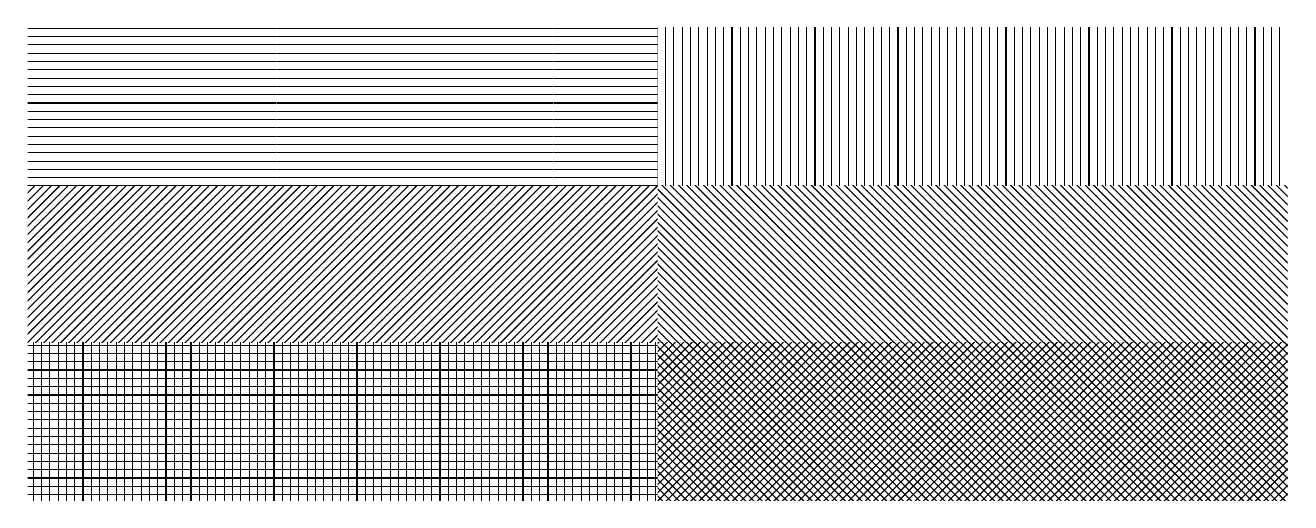
\begin{tikzpicture}
%横线%竖线
\fill[pattern = horizontal lines] (-8,0) rectangle (0,2);
\fill[pattern = vertical lines] (0,0) rectangle (8,2);

%斜线
\begin{scope}[yshift=-2cm]
\fill[pattern = north east lines] (-8,0) rectangle (0,2);
\fill[pattern = north west lines] (0,0) rectangle (8,2);
\end{scope}

%网格线 交叉线
\begin{scope}[yshift=-4cm]
\fill[pattern = grid] (-8,0) rectangle (0,2);
\fill[pattern = crosshatch] (0,0) rectangle (8,2);
\end{scope}




\end{tikzpicture}
\end{document}